\usetikzlibrary{arrows}
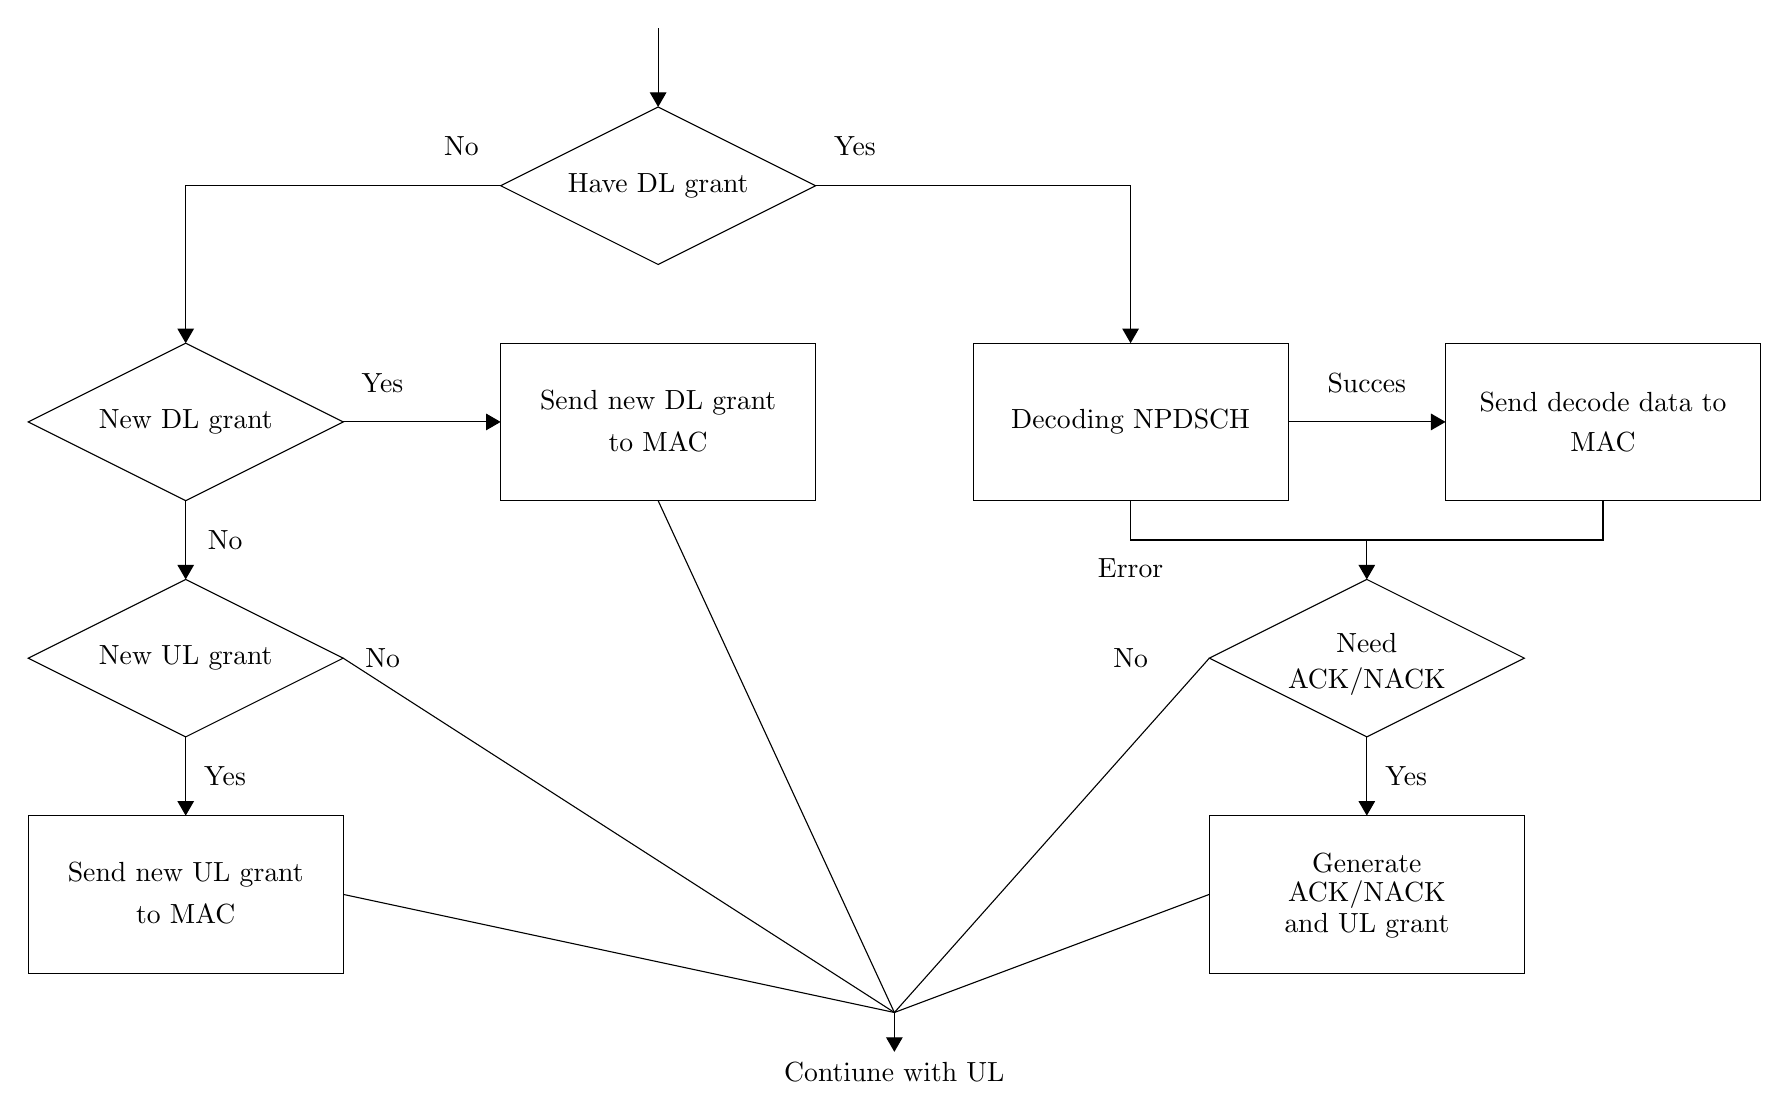
\begin{tikzpicture}

\draw (0,1) -- (-2,0) node (v2) {} -- (0,-1) -- (2,0) node (v7) {} -- (0,1) node (v15) {};
\draw (-6,-2)  -- (-8,-3) -- (-6,-4) node (v3) {} -- (-4,-3) node (v6) {} -- (-6,-2) node (v1) {};
\draw (-6,-5)  -- (-8,-6) -- (-6,-7) node (v5) {} -- (-4,-6) node (v8) {} -- (-6,-5) node (v4) {};
\draw  (4,-2) rectangle (8,-4);
\draw  (10,-2) rectangle (14,-4);
\draw  (7,-8) rectangle (11,-10);
\draw  (-2,-2) rectangle (2,-4);
\draw  (-8,-8) rectangle (-4,-10);
\draw [-triangle 60](-2,0) -- (-6,0) -- (-6,-2);
\draw [-triangle 60](-6,-4) -- (-6,-5);
\draw [-triangle 60](-6,-7) -- (-6,-8);
\draw [-triangle 60](-4,-3) -- (-2,-3);
\draw [-triangle 60](2,0) -- (6,0) -- (6,-2);
\draw [-triangle 60](8,-3) -- (10,-3);

\draw (0,-4) -- (3,-10.5) node (v9) {};
\node at (0,0) {Have DL grant};
\node at (-6,-3) {New DL grant};
\node at (-6,-6) {New UL grant};
\node at (0,-2.75) {Send new DL grant};
\node at (-6,-8.75) {Send new UL grant};
\node at (6,-3) {Decoding NPDSCH};
\node at (12,-2.75) {Send decode data to};
\node at (9,-8.6) {Generate};
\node at (3,-11.25) {Contiune with UL};
\node at (-6,-9.25) {to MAC};
\node at (9,-9.4) {and UL grant};
\node at (12,-3.25) {MAC};
\node at (0,-3.25) {to MAC};
\node at (-2.5,0.5) {No};
\node at (2.5,0.5) {Yes};
\node at (-3.5,-2.5) {Yes};
\node at (-5.5,-4.5) {No};
\node at (-3.5,-6) {No};
\node at (-5.5,-7.5) {Yes};
\node at (6,-4.85) {Error};
\node at (9,-2.5) {Succes};

\draw (-4,-6) -- (3,-10.5);
\draw (-4,-9) -- (3,-10.5);
\draw  -- (3,-10.5);
\draw (7,-9) -- (3,-10.5);
\draw [-triangle 60](3,-10.5) node (v12) {} -- (3,-11);
\draw (9,-5) node (v10) {} -- (7,-6) node (v11) {} -- (9,-7) node (v14) {} -- (11,-6) --  (9,-5) node (v13) {};
\draw (7,-6) -- (3,-10.5);
\draw [-triangle 60](9,-7) -- (9,-8);
\node at (9,-5.8) {Need};
\node at (9.5,-7.5) {Yes};
\node at (6,-6) {No};
\draw [-triangle 60](0,2) -- (0,1);
\draw [-triangle 60](6,-4) -- (6,-4.5) -- (9,-4.5) -- (9,-5);
\draw (12,-4) -- (12,-4.5) -- (8.5,-4.5);
\node at (9,-9) {ACK/NACK};
\node at (9,-6.3) {ACK/NACK};
\end{tikzpicture}